\documentclass[tikz, crop, border=5pt]{standalone}

\usepackage{xcolor}
\usepackage{mathtools}

\DeclareMathOperator{\uniform}{\mathcal{U}}

\usetikzlibrary{
    positioning,
    arrows.meta
}

\tikzset{%
    random variable/.style={%
        circle,
        draw,
        inner sep = 0pt,
        outer sep = 0pt,
        minimum width=1cm
    },
    state/.style={%
        circle,
        draw,
        inner sep = 0pt,
        outer sep = 0pt,
        minimum width=1cm,
        fill=black!20
    },
    observed rv/.style={%
        random variable,
        fill=blue!20,
    },
    unobserved rv/.style={%
        random variable,
        fill=white,
    },
    arrow/.style={%
        >={Stealth[round]},
    },
    formula/.style={%
        rectangle,
        draw=gray,
        rounded corners=2pt,
        inner sep = 2pt,
        outer sep = 0pt,
        minimum width=12cm,
        minimum height=1cm,
    },
}

\begin{document}
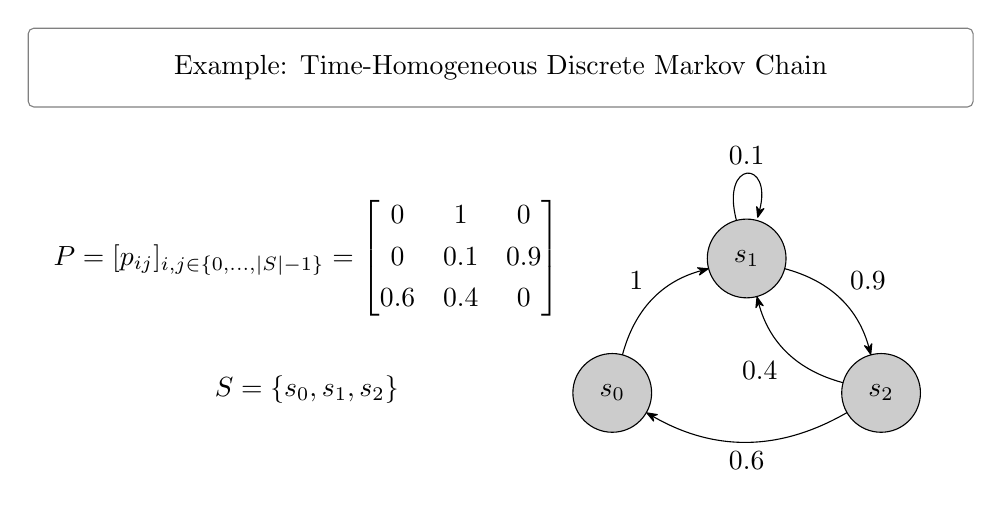
\begin{tikzpicture}
    \node[formula] (title) {Example: Time-Homogeneous Discrete Markov Chain};

    \node[below=of title] (anchor) {};

    \node[state, right=of anchor, xshift=1.5cm, yshift=-0.8cm] (S1) {$s_1$};
    \node[state, below left= of S1] (S0) {$s_0$};
    \node[state, below right= of S1] (S2) {$s_2$};

    \draw (S0) edge[arrow, ->, bend left] node[auto] {1} (S1);
    \draw (S1) edge[arrow, ->, loop above] node[auto] {0.1} (S1);
    \draw (S1) edge[arrow, ->, bend left] node[auto] {0.9} (S2);
    \draw (S2) edge[arrow, ->, bend left]node[auto] {0.4} (S1);
    \draw (S2) edge[arrow, ->, bend left] node[auto] {0.6} (S0);

    \node[left=of anchor, xshift=2cm, yshift=-0.8cm] (transition) {$P = [p_{ij}]_{i,j \in \{0, \dots, |S|-1\}} = \begin{bmatrix} 0 & 1 & 0\\[0.3em]
                      0 & 0.1 & 0.9\\[0.3em]
                      0.6 & 0.4 & 0 \end{bmatrix}$};
    \node[below=of transition, yshift=0.5cm] (states) {$S= \{ s_0, s_1, s_2\}$};
\end{tikzpicture}
\end{document}